\documentclass[11pt,a4paper]{../tutorial}
\usepackage[hidelinks]{hyperref}


\usepackage{lstlinebgrd}
\usepackage{listings}
\usepackage{ifthen}

\title{Tutorial 11 --- Building Controllers in PVSio-Web}
\date{April 2019}
\author{Maurizio Palmieri}

\begin{document}

\section*{Overview}

This tutorial will help you to:

\begin{enumerate}[noitemsep]
\item Install PVSio-web
\item Generate a  controller using PVSio-Web
\item Generate an FMU from a PVSio-Web project
\item Prepare an ARDUINO Sketch with the FMU code 
\item Compile and upload the Sketch into the robot 
\end{enumerate}

\section*{Requirements}

This tutorial requires the following tools:

\begin{itemize}[noitemsep]
\item Linux OS (or a VM with Linux as OS)
\item INTO-CPS Application
\item COE (Co-simulation Orchestration Engine) accessible to the Application
\item ARDUINO IDE (1.8.5) 
\item avr-gcc (GCC) $\geq$ 6.3.0
\item avr-g++ (GCC) $\geq$ 6.3.0   

\end{itemize}




\section{Downloading the VM (for Windows users only)}
\begin{instructions}
\item Go to the following link: \url{http://releases.ubuntu.com/16.04/} , and select the desktop image that fits your machine.
\item Launch Virtual Box
\item Click New, give a name to the machine, e.g., PVSClass2019, its type is Linux, and its version Ubuntu. Click Continue.
\item Select Create a virtual hard drive file and use default options.
\item  Start the new virtual machine
\item Follow the instructions to install Ubuntu.

\end{instructions}
\section{Installation of PVSio-web}
\begin{instructions}
\item Type "sudo apt-get install npm" and "sudo apt-get install nodejs-legacy" on terminal to install Nodejs.
\item Type "git clone https://github.com/mapalmieri/pvsio-web" to download the folder pvsio-web
\item Move into the pvsio-web folder (type "cd pvsio-web")
\item Type "npm install" (it will require few minutes to complete)

\end{instructions}
\section{Make a PVSio-web Project}
\begin{instructions}
\item Launch the script start.sh (type "./start.sh")
\item Then open a web browser and go to the page "http://localhost:8082/"
\item On the web page, click on New Project in the topbar and name it \emph{LFRController}.
\item On the topbar of the project click "Save Project" 

\end{instructions}
\section{Adding variables to an Emuchart diagram}
\begin{instructions}
\item Then on the right panel, click on the on/off button next to "EmuCharts Editor".
\item \label{VARIABLES}  Then scroll down untill you see a new bar and click on \emph{VARIABLES}
\begin{figure}[h]
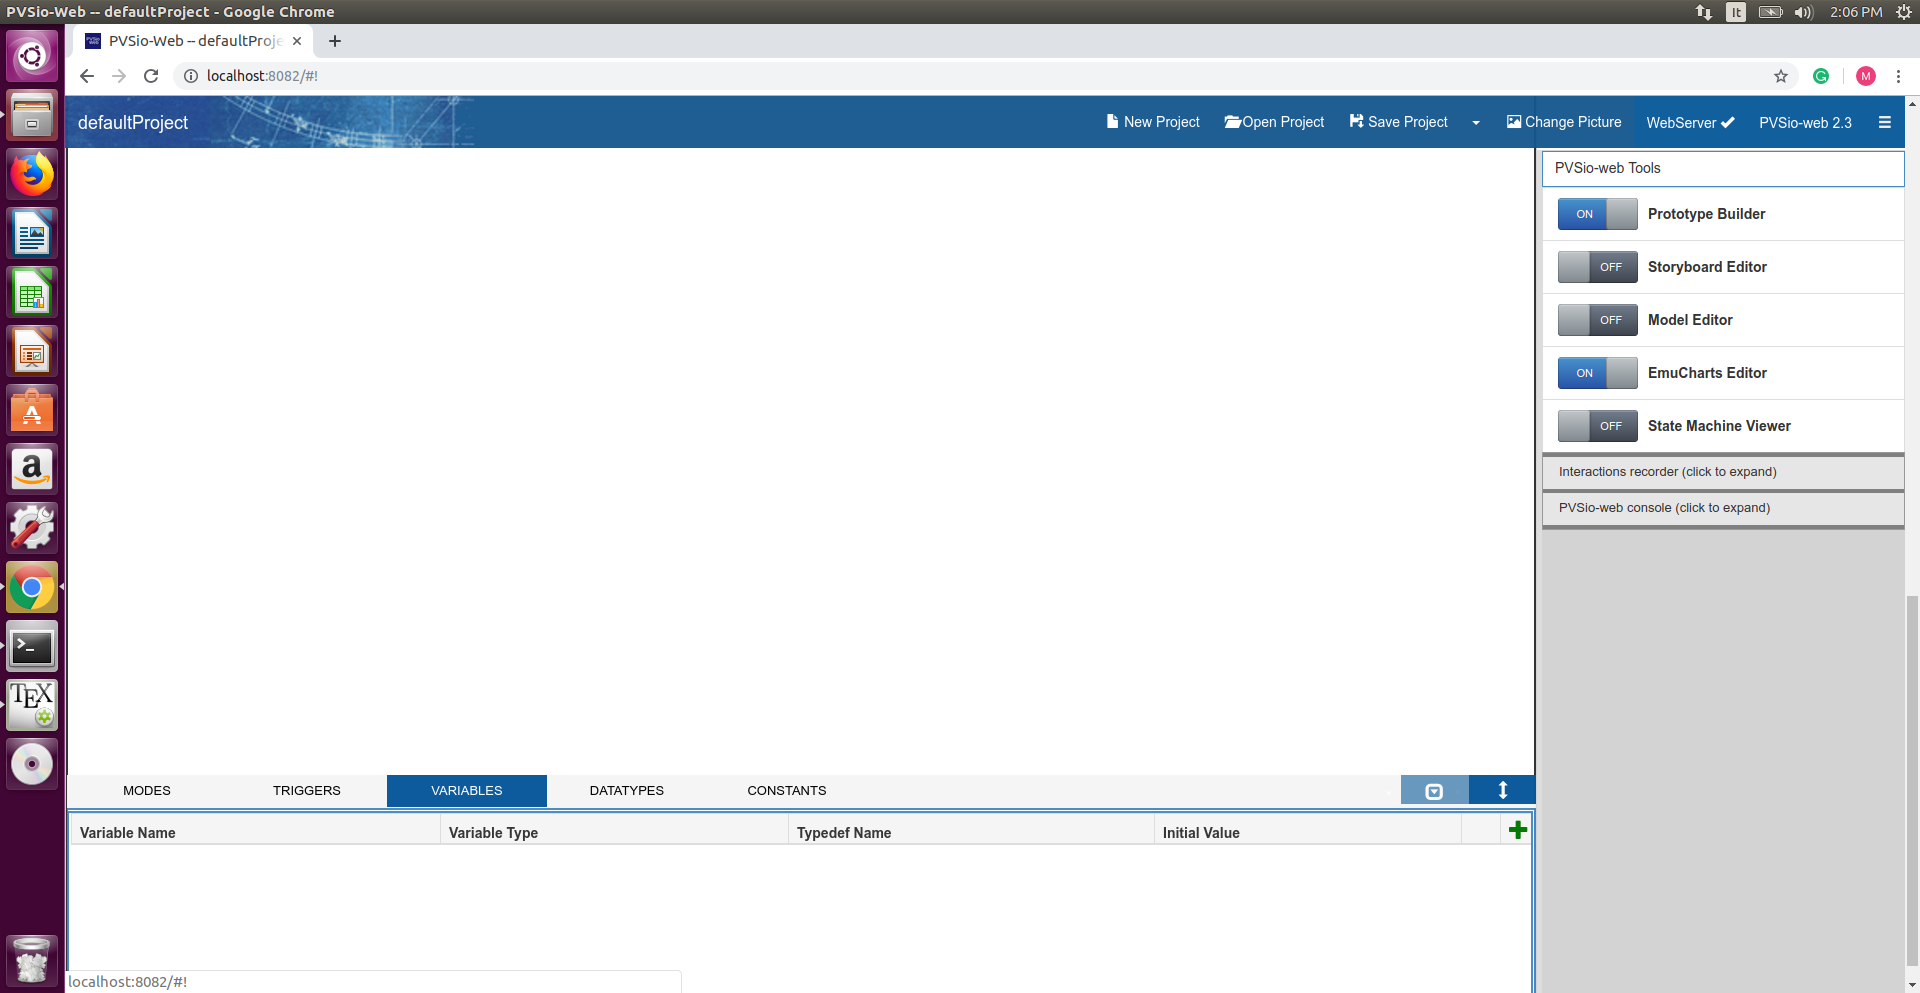
\includegraphics[width=1\textwidth]{figures/VARIABLES.png}
\label{figVARIABLES}
\caption{Figure for  \ref{VARIABLES}}
\end{figure}
\item \label{LeftSensor}Click on the green + on the right
\begin{enumerate}
\item Choose a representative name, such as "LeftSensor"
\item This is a "real" variable
\item "Typedef name" is the type used in the MISRA C code, choose float64\_ t
\item Initial value "0"
\item Scope Input
\end{enumerate}
\begin{figure}[h]
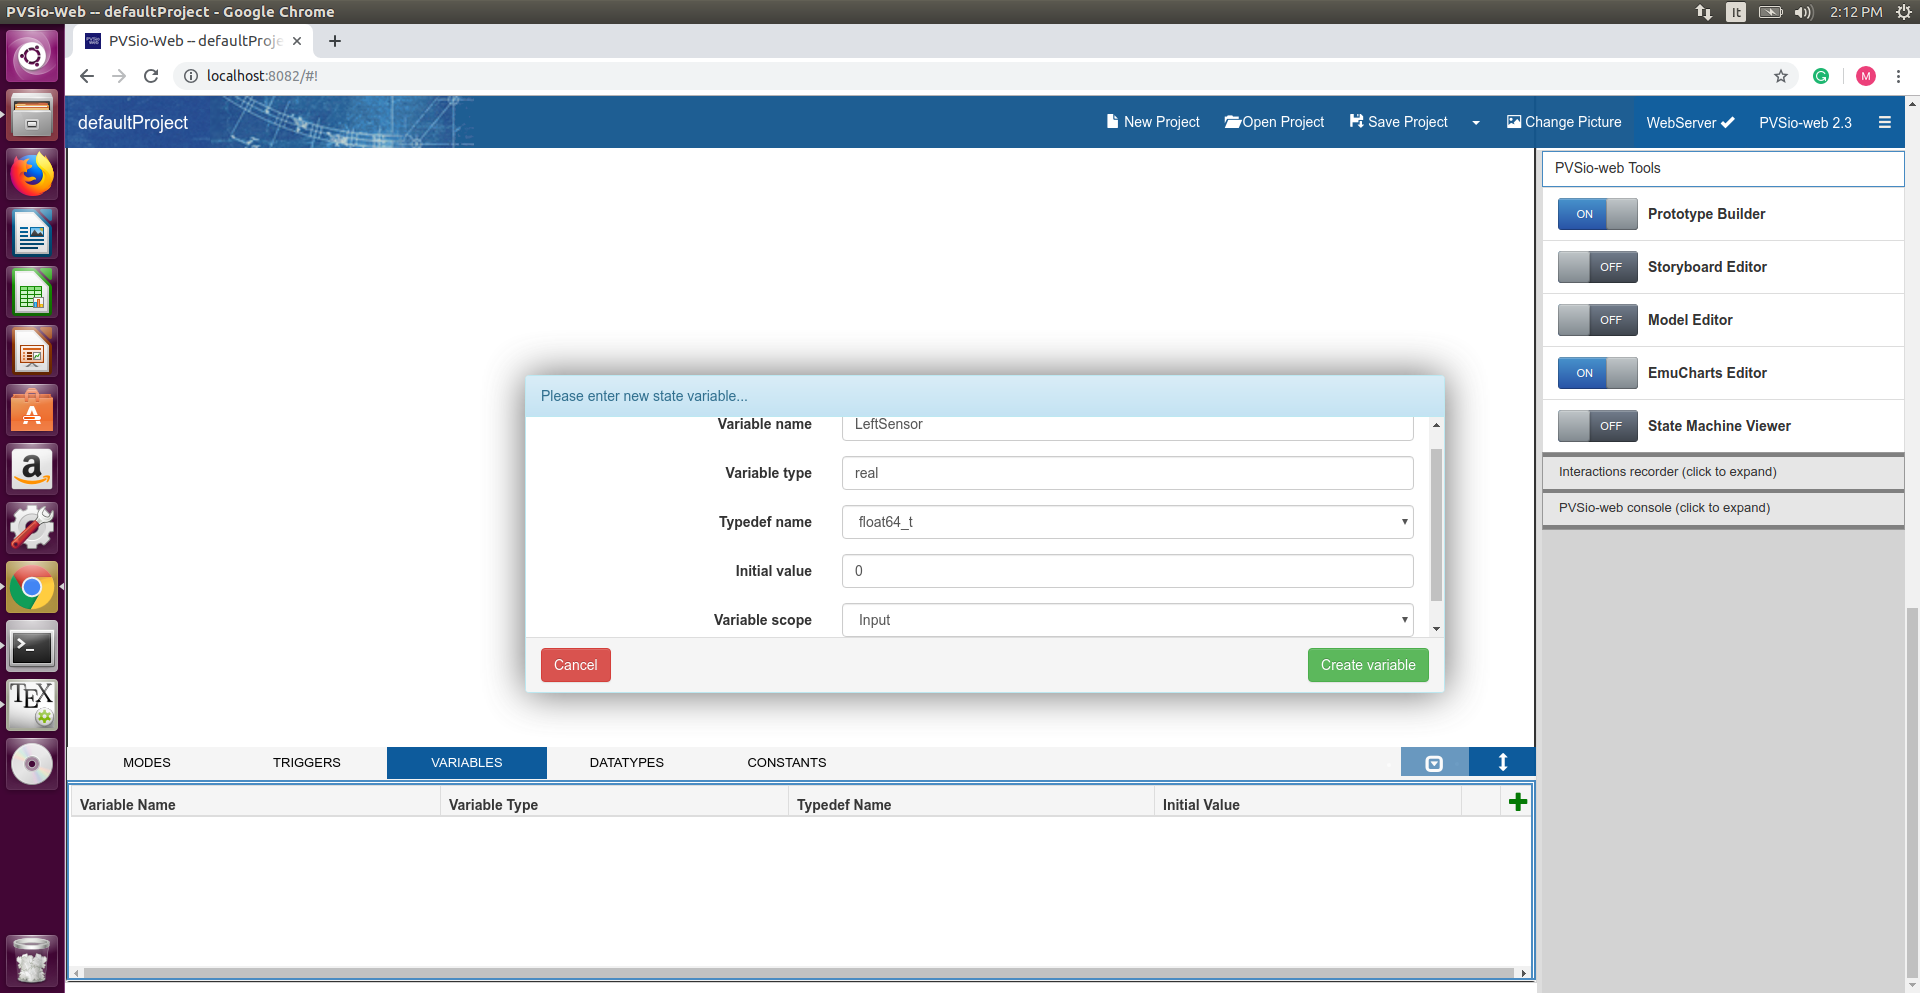
\includegraphics[width=1\textwidth]{figures/LeftSensor.png}
\label{}
\caption{Figure for  \ref{LeftSensor}}
\end{figure}

\item Repeat for RightSensor, LeftServo(Scope: output) and RightServo (Scope: output)
\item Scroll up to the Emucharts Editor bar
\item \label{Save1}On the bar, hover on File , then click on Save Chart
\begin{figure}[h]
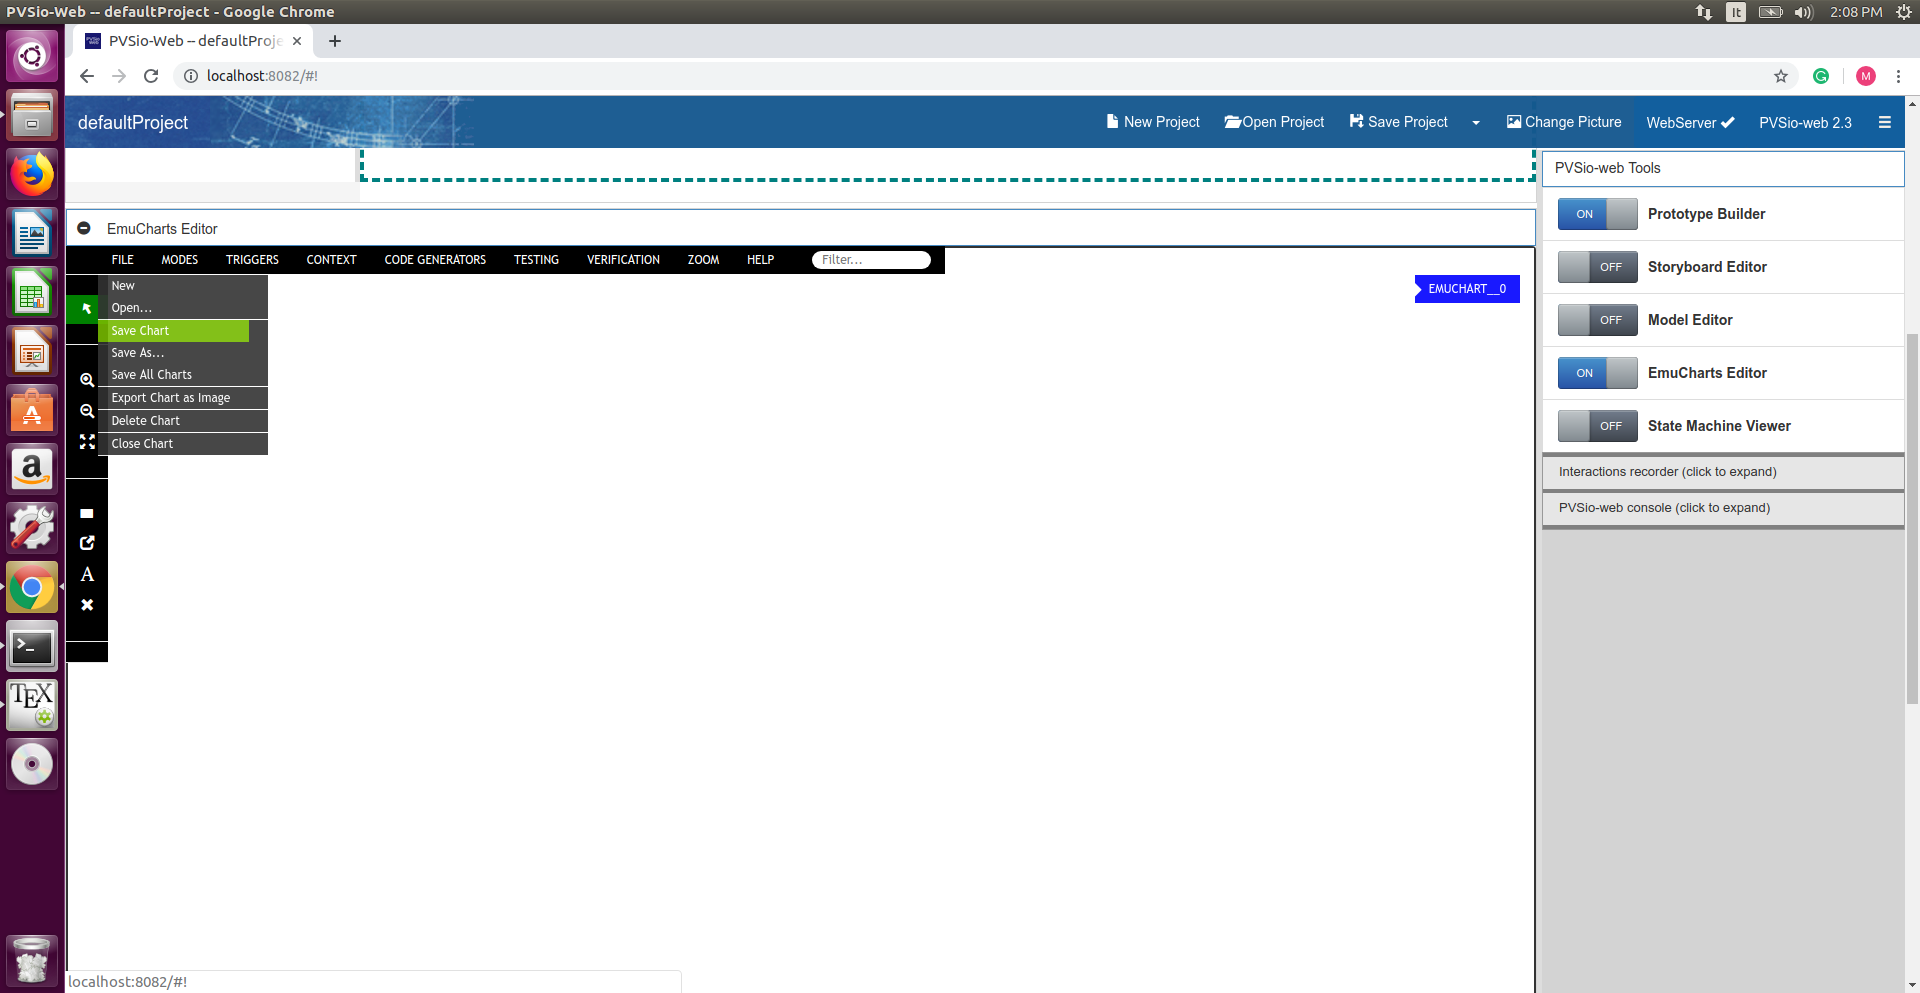
\includegraphics[width=1\textwidth]{figures/Save_Chart.png}
\caption{Figure for  \ref{Save1} and \ref{Save2}}
\end{figure}
\item On the topbar of the project click "Save Project"

\end{instructions}
\section{Creating the Emuchart diagram}
\begin{instructions}
\item On the left panel click on "Add modes" and then click on the middle section to place the mode.
\item On the left panel click on "Browse diagram" then double-click on the newly created mode and name it "Auto"
\item On the left panel click on "Add trigger", then click on the mode Auto to add a reentrant edge
\item On the left panel click on "Browse diagram" then double-click on the newly created trigger and copy the following snippet:
\begin{verbatim}
tick
[LeftSensor <= 150 AND RightSensor <= 150]
{LeftServo := 0.4;RightServo := -0.4}
\end{verbatim}

This transition drives the robot forward when both sensors see the painted line (sensor value less than or equal to 150).
\item Create another reentrant transition named "tick" for turning right when only the right sensor sees the painted line (\textbf{Hint:} to turn right LeftServo should be 0.5 and RightServo should be -0.1 )
\item Create another reentrant transition named "tick" for turning left when only the left sensor sees the painted line (\textbf{Hint:} to turn left LeftServo should be 0.1 and RightServo should be -0.5)
\item \label{Save2} On the bar, hover on File , then click on Save Chart
\item On the topbar of the project click "Save Project"


\end{instructions}
\section{Generating an FMU from Emuchart}
\begin{instructions}
\item \label{FMIPackage} Hover on "CODE GENERATORS" then click on "FMI Package"
\begin{figure}[h]
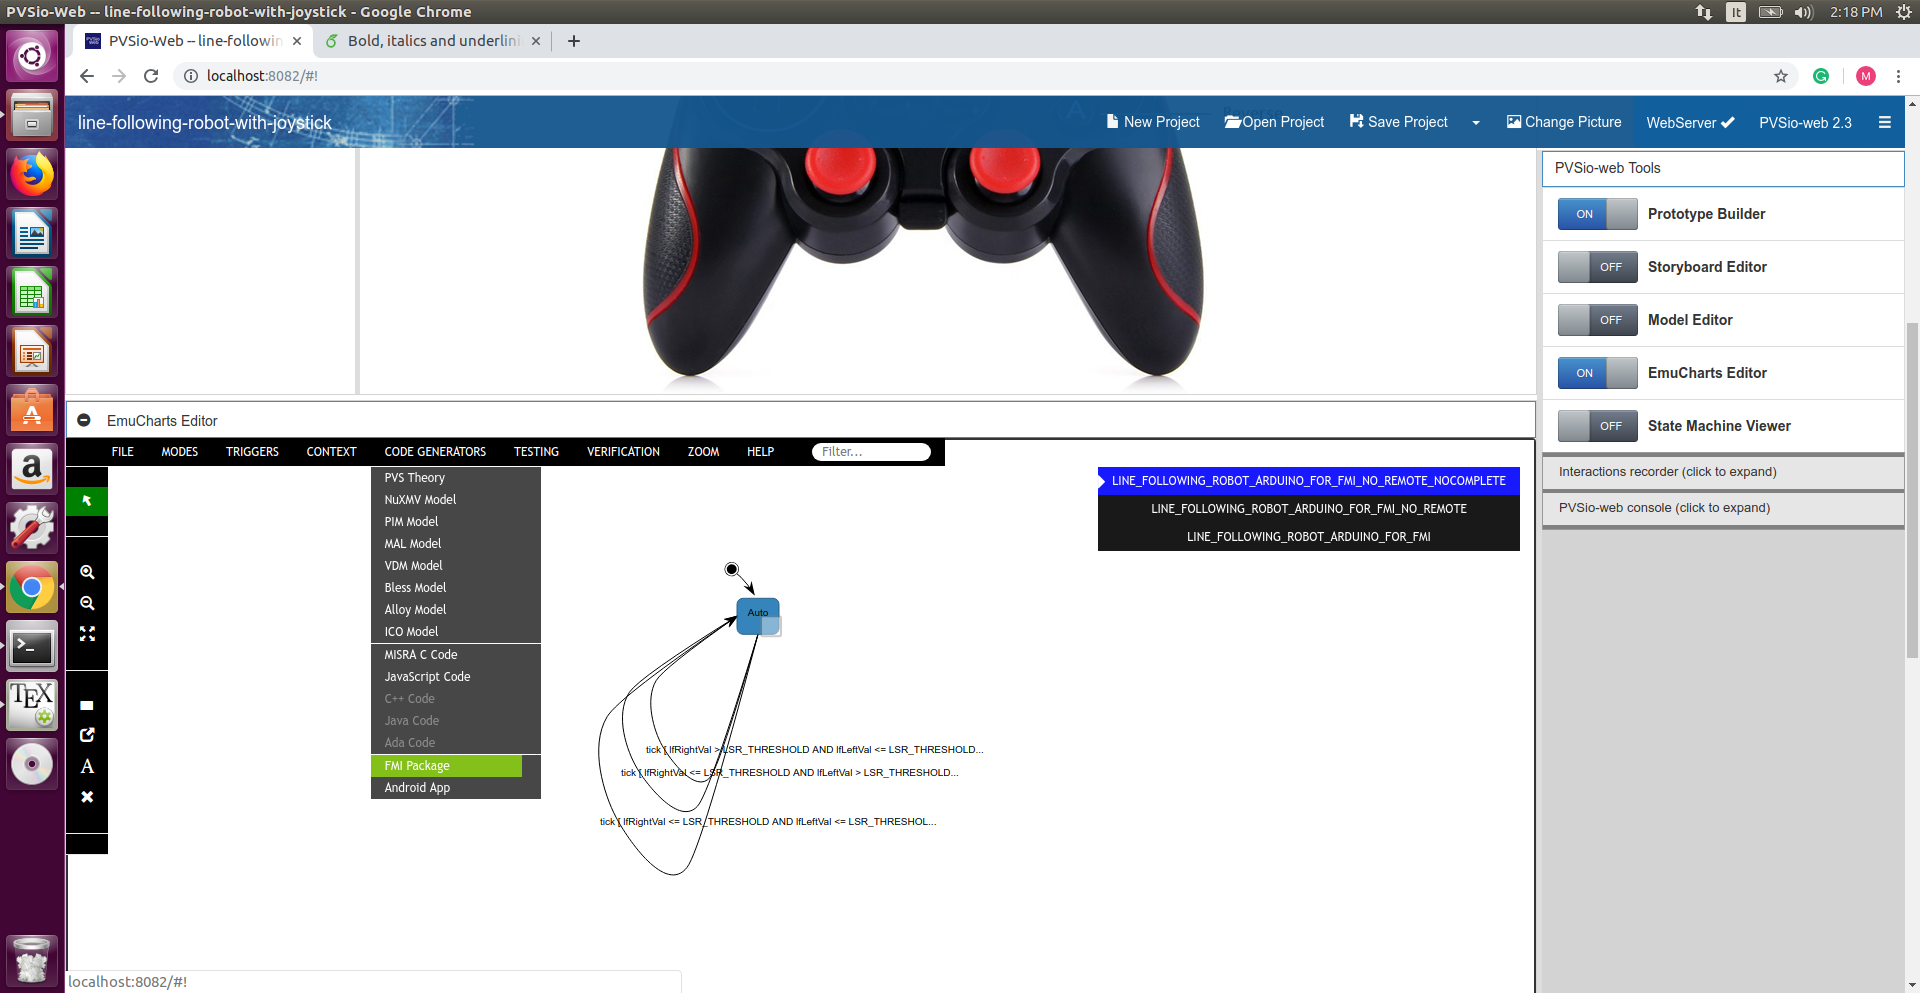
\includegraphics[width=1\textwidth]{figures/FMIPackage.png}
\caption{Figure for \ref{FMIPackage}}
\end{figure}
\item The files for the FMU have been generated in the fmu-pvs folder, located in the folder pvsio-web/examples/projects/LFRController along with a makefile. Open a terminal into the fum-pvs folder, and type "make all" on the terminal.

\section{INTO-CPS co-simulation}
\item Open INTO-CPS application
\item File -- Import example project; select the line follower robot case study.
\item Move the fmu generated with PVSio-web into the FMU folder of the project.
\item Modify the non-3d multimodel to use the new FMU instead of the one in overture.
\end{instructions}

\section{Arduino setup}
\begin{instructions}
\item Download the ARDUINO IDE version 1.8.5 from:\\
	\url{https://www.arduino.cc/en/Main/Software}.  Choose the zip file
	version and extract the folder into your
	\texttt{into-cps-projects/install} folder. (Choose the respective files in the case of Linux or macOS installations)
	
\item The current C/C++ compiler version shipped in the ARDUINO IDE is prior to the required 6.3. So one needs to install an updated version. You can find one from:\\
	\url{http://blog.zakkemble.co.uk/avr-gcc-builds/}. 
	
	Download and unzip it into your  \texttt{into-cps-projects/install} folder. (Choose the respective files in the case of Linux or macOS installations)
	
\section{Create the FMU and upload to Arduino (Linux/macOS Only)}


\item Go back to the PVSio-web page and open the project line\_ following\_ robot: in the topbar click on Open Project, scroll down to the line\_ following\_ robot (\textbf{avoid line\_ following\_ robot1 !!}) and click open.
\item Open the Emuchart Editor, hover on "CODE GENERATORS" then click on "FMI Package".
\item Before creating the FMU we need to apply two small modifications:
 in skeleton.c , misrac/line\_ following\_ robot.c and  misrac/line\_ following\_ robot.h change the name "init" with "Init" \textbf{the different is the capital letter}.
\item type "make all" on the terminal

\item Connect robot to USB and find port (for example you may find /dev/ttyACM0 after running \verb'ls /dev/' ). \textbf{if you don't have the robot or the cable assume that you can use /dev/ttyACM0. When you have the robot please confirm this step}



	
	

\item In a terminal change to the \emph{tutorial\_10/Deploy/linux} folder. In it you should find the files: \emph{main.cpp}, \emph{modeldescription.h} and the \emph{deploy.sh} script.

\item Set the following variables used in the \emph{deploy.sh} script adapting the path to your own choices:
	\begin{itemize}
		\item port - to the previous result 
		\item gcc\_path - to into\_cps\_project/install/avr-gcc-8.3.0-x64-linux/bin 
		\item avr - to into\_cps\_project/install/arduino-1.8.5/hardware/arduino/avr/ 
		\item avrdudeconfig - to into\_cps\_project/install/arduino-1.8.5/hardware/tools/avr/etc/avrdude.conf
	\end{itemize}
\item Make the following changes to main.cpp
	\begin{itemize}
		\item in line 10, change Fmu.h with fmu.h
		\item comment line 11 (the other include)
		\item comment line 121 (LSR\_ THRESHOLD)
	\end{itemize}
\item Move the newly created FMU in this folder.
\item Run the \emph{deploy.sh} script with  line\_ follower\_ robot.fmu as a parameter. 
\end{instructions}



\end{document}
